\documentclass[a4paper,11.5pt]{article}
\usepackage[textwidth=170mm, textheight=230mm, inner=20mm, top=20mm, bottom=30mm]{geometry}
\usepackage[normalem]{ulem}
\usepackage[utf8]{inputenc}
\usepackage[T1]{fontenc}
\PassOptionsToPackage{defaults=hu-min}{magyar.ldf}
\usepackage[magyar]{babel}
\usepackage{amsmath, xcolor, amsthm,amssymb,paralist,array, ellipsis, graphicx, tikz}
\usetikzlibrary{shapes.geometric, arrows}
%\usepackage{marvosym}

\usepackage{listings}
\lstset{
	language=C++, 
	basicstyle=\ttfamily, 
	keywordstyle=\color{blue}\ttfamily, 
	stringstyle=\color{red}\ttfamily,
	tabsize = 4
}

\makeatletter
\renewcommand*{\mathellipsis}{%
	\mathinner{%
		\kern\ellipsisbeforegap%
		{\ldotp}\kern\ellipsisgap%
		{\ldotp}\kern\ellipsisgap%
		{\ldotp}\kern\ellipsisaftergap%
	}%
}
\renewcommand*{\dotsb@}{%
	\mathinner{%
		\kern\ellipsisbeforegap%
		{\cdotp}\kern\ellipsisgap%
		{\cdotp}\kern\ellipsisgap%
		{\cdotp}\kern\ellipsisaftergap%
	}%
}
\renewcommand*{\@cdots}{%
	\mathinner{%
		\kern\ellipsisbeforegap%
		{\cdotp}\kern\ellipsisgap%
		{\cdotp}\kern\ellipsisgap%
		{\cdotp}\kern\ellipsisaftergap%
	}%
}
\renewcommand*{\ellipsis@default}{%
	\ellipsis@before
	\kern\ellipsisbeforegap
	.\kern\ellipsisgap
	.\kern\ellipsisgap
	.\kern\ellipsisgap
	\ellipsis@after\relax}
\renewcommand*{\ellipsis@centered}{%
	\ellipsis@before
	\kern\ellipsisbeforegap
	.\kern\ellipsisgap
	.\kern\ellipsisgap
	.\kern\ellipsisaftergap
	\ellipsis@after\relax}
\AtBeginDocument{%
	\DeclareRobustCommand*{\dots}{%
		\ifmmode\@xp\mdots@\else\@xp\textellipsis\fi}}
\def\ellipsisgap{.1em}
\def\ellipsisbeforegap{.05em}
\def\ellipsisaftergap{.05em}
\makeatother

\usepackage{hyperref}

\begin{document}
	%%%%%%%%%%%RÖVIDÍTÉSEK%%%%%%%%%%
	\setlength\parindent{0pt}
	\def\s{\hspace{0.2mm}\vphantom{\beta}}
	\def\Z{\mathbb{Z}}
	\def\Q{\mathbb{Q}}
	\def\R{\mathbb{R}}
	\def\C{\mathbb{C}}
	\def\N{\mathbb{N}}
	\def\Ra{\overline{\mathbb{R}}}
	
	\def\sume{\displaystyle\sum_{n=1}^{+\infty}}
	\def\sumn{\displaystyle\sum_{n=0}^{+\infty}}
	
	\def\narrow{\underset{n\rightarrow+\infty}{\longrightarrow}}
	\def\limn{\displaystyle\lim_{n\to +\infty}}
	\def\limx{\displaystyle\lim_{x\to +\infty}}
	
	\theoremstyle{definition}
	\newtheorem{theorem}{Tétel}[subsection] 
	
	\theoremstyle{definition}
	\newtheorem{definition}[theorem]{Definíció} 
	\newtheorem{example}[theorem]{Példa} 
	\newtheorem{task}[theorem]{Feladat} 
	\newtheorem{note}[theorem]{Megjegyzés}
	%%%%%%%%%%%%%%%%%%%%%%%%%%%%%%%%%%%%%%%%%%%%%%%%%%%%%%%%%%%%%%%%%%%%%
	\begin{center}
		{\LARGE\textbf{C++}}
		
		{\Large Gyakorlat jegyzet}
		
		5. óra.
	\end{center}
	A jegyzetet \textsc{Umann} Kristóf készítette \textsc{Horváth} Gábor  előadásán. (\today)
	\section{A c++ memóriamodellje}
	A c++ szabvány 3 memóriatípust különít el. Ezek közül a stack-et használtuk csak eddig.
	\begin{center}
		\begin{tabular}{|c|}
			\\
			\\
			\\
			\\
			stack\\
			\\
			\hline
		\end{tabular}\quad 
		\begin{tabular}{|c|}
			\hline
			\quad \quad \\
			\\
			Globális/statikus\\
			\\
			\hline
		\end{tabular}\quad 
		\begin{tabular}{|c|}
			\hline
			\quad \quad \\
			\\
			Heap/free storage\\
			\\
			\hline
		\end{tabular}
	\end{center}
	\subsection{Stack}
	A stack a c++ alapértelmezett ,,memóriája'', minden változó alapértelmezetten itt jön létre és semmisül meg. Ez utóbbi nagyon fontos: azok a változók, amelyek kiesnek a scope-ból, automatikusan megsemmisülnek, így nem kell a létrehozással és a megsemmisüléssel külön bajlódnunk.
	
	\begin{lstlisting}
#include <iostream>

int f()
{
	int x = 0; //x letrejon
	++x;
	return x;
} //x megsemmisul

int main()
{
	std::cout << f() << std::endl;
	std::cout << f() << std::endl;
	std::cout << f() << std::endl;
	std::cout << f() << std::endl;
	std::cout << f() << std::endl;
}
	\end{lstlisting}
	Kimenet: \texttt{1 1 1 1 1}
	
	A stack-en létrehozott változókat szokás \textbf{automatikus változók}nak (\textit{automatic variable}) is hívni.
	
	\smallskip
	A stacken lérehozott változók kezelése nagyon kényelmes, mert jól látható, mikor jönnek jönnek létre, mikor semmisülnek meg, stb. Azonban fordulhat elő olyan, hogy nem szeretnénk, hogy minden alkalommal megsemmisüljön a fenti példában az \texttt{x}, ilyenkor kiút lehet a statikus változók használata.
	\subsection{Globális/statikus tárhely}
	%TODO globális változók
	Írjuk át a fenti \texttt{f} függvényt, hogy \texttt{x} ne automatikus, hanem \textbf{statikus változó} (\textit{static variable}) legyen!
	\begin{lstlisting}
int f()
{
	static int x = 0;
	++x;
	return x;
}

int main(){/* */}
	\end{lstlisting}
	Kimenet: \texttt{1 2 3 4 5}
	
	Ebben az esetben azonban a függvény első hivásától a program futásának végéig benne marad a memóriában az \texttt{x}, így mindig egyre nagyobb számokat ad majd \texttt{f()} vissza.
	\begin{note}
		Nem igazán szeretjük a \texttt{static} változókat. Például a multithread programok különösen tudnak szenvedni tőle, mert nehéz, vagy lehetetlen átlátni, hogy mikor mire változik az értékük.
	\end{note}
	Amennyiben azt szeretnénk hogy \texttt{x} ne is semmisüljön meg azonnal, de statikus se legyen, létrehozhatjuk úgy, hogy a megsemmisítéséről is nekünk kell gondoskodni.
	\subsection{Heap/free storage}
	A heap-en létrehzoott változókat \textbf{dinamikus változók}nak (\textit{dynamic variable}) is szokás szokás hívni. A heap segítségével nagyon nagy szabadságra tehetünk szert, azonban ez a szabadság kötelességekkel is jár.
	\begin{lstlisting}
int main()
{
	int *p = new int(5);
	delete p;
}
	\end{lstlisting}
	Fentebb láthatjuk hogyan lehet egy változót a heap-en létrehozni. Ehhez használatos a \texttt{new} operátor, a heapen lefoglalandó memória típusa (ez esetben \texttt{int}), és konstruktor paraméterek (itt példaképp 5 kezdőértékkel inicializálink). Fontos, hogy a stack-et teljesen nem kerültük meg, mert szükségünk van egy pointerre, mely a heap-en kezelt címre mutat (\texttt{p}).
	
	Ezt a címet a \texttt{delete} operátorral tudjuk felszabadítani.
	\begin{center}
		
		\begin{tabular}{|c|}
			\\
			\\
			\quad \quad \quad \quad \quad \\
			p\\
			\\
			\\
			\hline
		\end{tabular}\quad*nyilacska \texttt{p}-ből a benti négyzetre*
		\begin{tabular}{|c|}
			\hline
			\quad \quad\quad \quad \quad \quad  \\
			\quad \quad \fbox{5}\\
			\\
			\hline
		\end{tabular}
	\end{center}
	
	A heapen nincs a változóknak nevük, így mindig szükségünk lesz egy mutatóra, hogy tudjunk rá hivatkozni. \textbf{Ha egyszer létrehozunk valamit a heap-en, nekünk is kell gondoskodni arról, hogy felszabadítsuk.} Az egyik leggyakoribb hiba a dinamikus memóriakezelésnél, ha a memóriát nem szabadítjuk fel, ilyenkor a lefoglalt memóriaterületre hivatkozni már nem lehet de lefoglalva marad, mondhatni elszivárog (\textit{memory leak}). 
	\smallskip
	
	Bár az operációs rendszer erre szokott figyelni, és megpróbál minden, a program által lefoglalt memóriát felszabadítani a dutás befejeztével, de nem mindenható, előfordulhat hogy ez nem elég teljeskörú, és ilyenkor az a memóriaterületek újraindításig lefoglalva maradnak.
	\medskip
	
	A dinamikus lefoglalt memória szabályos felszabadítását számos dolog nehezíti. Fényes példa erre a kivételkezelés, melynél hamarabb félbreszakítódik a függvény mintsem hogy felszabadítson minden memóriát. Azonban ha nagyon ügyelünk erre, előfordulhat hogy nem figyelünk, és egy memóriaterületet kétszer szabadítunk fel, ami nem definiált viselkedés.
	\medskip
	
	Előfordulhat, hogy egy már felszabadított memóriaterületre akarunk írni. Sajnos iylen hibát könnyű ejteni, hisz a \texttt{delete} a \texttt{p} által mutatott memóriaterületet, nem a \texttt{p}-t fogja törölni.
	\begin{note}
		A nullpointer törlésekor nem történik semmi (\textit{no-op}).
	\end{note}
	\begin{note}
		Amint elvesztettük az utolsó mutatót, ami egy adott lefoglalt memóriacímre mutat, az közel garantáltan elszivárgott memória. A szabvány nem foglal magában semmilyen lehetőséget ezeknek a visszaszerzésére (és könnyen látható, hogy ha meg is oldjuk, a szabványtól függetlenül hogy ezeket a memóriacímeket összevadásszuk, az igen költséges lenne).
	\end{note}
	Láthatjuk, hogy a heap használata macerás, hibaforrásokkal teli, ráadásul az allokálás (memória lefoglalás) még lassabb is. De miért használjuk mégis? Nos, ha egy mód van rá, ne tegyük. Ha meg lehet oldani, hogy a stack-en el tudjunk tárolni valamit, tegyük azt. A stacken azonban nem lehet mindent létrehozni, továbbá nagyon véges, hamar be tud telni (\textit{stack overflow}), illetve kevésbé tudjuk kontrollálni a memóriát. A heap-en e téren sokkal nagyobb a szabadságunk.
	\section{Osztályok felépítése}
	A következő pár gyakorlaton egy láncolt listát fogunk implementálni, mely jól demonstrálja majd a dinamikus memóriakezelés veszélyeit is.
	
	\smallskip
	A láncolt lista egy olyan konténer, melynek minden eleme egy olyan listaelem, mely tartalmaz egy mutatót és (legalább egy) adatot tároló objektumot. A listaelem mutatója rámutat a lista következő elemére, és az utolsó elem pointere pedig egy nullpointer.
	\begin{center}
		\begin{tabular}{|c|c|}
			\hline
			\texttt{data}&\texttt{*next}\\
			\hline
		\end{tabular}
		\smallskip
		
		Egy listaelem.
		\medskip
		
		\begin{tabular}{|c|c|}
			\hline
			\texttt{8}&\texttt{}\\
			\hline
		\end{tabular}$\rightarrow$
		\begin{tabular}{|c|c|}
			\hline
			\texttt{7}&\texttt{}\\
			\hline
		\end{tabular}$\rightarrow$
		\begin{tabular}{|c|c|}
			\hline
			\texttt{2}&\texttt{$\emptyset$}\\
			\hline
		\end{tabular}
		\smallskip
		
		3 elemű láncolt lista.
	\end{center}
	\subsection{Struct-ok}
	Egy láncolt lista elemét implementálhatjuk pl. így:
	\begin{lstlisting}
struct List
{
	int data;
	List *next
};
	\end{lstlisting}
	Alkalmazzuk is ezt úgy, hogy  a listaelemek dinamikusan legyen eltárolva!
	\begin{lstlisting}
int main()
{
	List *head = new List;
	head->data = 8; //(*head).data   ==   head->data
	head->next = new List;
	
	head->next->data = 7;
	head->next->next = new List;
	
	head->next->next->data = 2;
	head->next->next->next = NULL;
	
	delete head;
	delete head->next;
	delete head->next->next;
}
	\end{lstlisting}
	Ezen a ponton mondhatjuk azt hogy készen vagyunk, hisz \texttt{List} használható láncolt listaként (bár valóban igen kényelmetlen).
	\medskip
	
	\begin{center}
		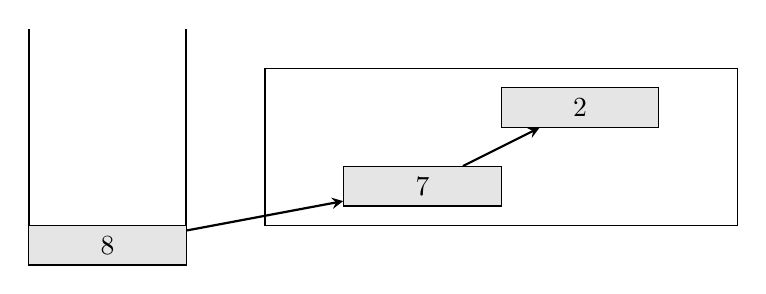
\begin{tikzpicture}
		\tikzstyle{Heap} = [rectangle, minimum width=6cm, minimum height=2cm, text centered, draw=black, fill=white]
		\tikzstyle{Stack} = [rectangle, minimum width=3cm, minimum height=1cm, text centered, draw=black, fill=white]
		\tikzstyle{ListNode} = [rectangle, minimum width=2cm, minimum height=5mm, text centered, draw=black, fill= gray!20]
		\tikzstyle{arrow} = [thick,->,>=stealth]
		
		%\foreach \x in {-2,-1,0,1,2,3,4}
		%	\draw (\x cm,1pt) -- (\x cm,-1pt) node[anchor=north] {$\x$};
		%\foreach \y in {-2,-1,0,1,2,3,4}
		%	\draw (1pt,\y cm) -- (-1pt,\y cm) node[anchor=east] {$\y$};
		%\draw[step=5mm,gray,very thin] (-2,-2) grid (6,6);
		
		\draw [thick, black] (-3, 0) -- (-1, 0);
		\draw [thick, black] (-3, 0) -- (-3, 3);
		\draw [thick, black] (-1, 0) -- (-1, 3);
		\node[Heap] at (3,1.5){};
		\node (7node) [ListNode] at (2,1) {7};
		\node (2node) [ListNode] at (4,2) {2};
		\node (headNode) [ListNode] at (-2,0.25) {8};
		\draw [arrow] (7node) -- (2node);
		\draw [arrow] (headNode) -- (7node);
		\end{tikzpicture}
	\end{center}
	Sajnos a törlést sikerült picit elcsesznünk: először kitörljük a fejelemet (mely az első elemre mutat), viszont az első elem segítségével tudnánk a többi elemre is hivatkozni, így mire a második listaelemet törölnénk, \texttt{head} már egy felszabadított memóriaterületre mutat, amit törlés utáni használatnak (\textit{use after delete}) szokás nevezni, és az egy nem definiált viselkedés.
	
	A megoldás:
	\begin{lstlisting}
delete head->next->next;
delete head->next;
delete head;
	\end{lstlisting}
	\begin{note}
		A heap-en arra is figyelni kell, hogy jó sorrendben szabadítsuk fel a dolgokat. Könnyen lábonlőhetjük magunkat azzal, hogy egy kitörlünk valamit, ami hivatkozik egy másik memóriacímre, így azt a címet vagy elleakeljük, vagy ráhivatkozással nem definiált viselkedésbe keveredünk.
	\end{note}
	A változók a stacken fordított sorrendben semmisülnek meg, pont emiatt.
	\medskip
	
	Ez a ,,láncolt lista'' eddig eléggé gyér. A fő baj az, hogy nagyon sokat kell írni, méghozza lényegében ugyanazt, és nem feltétlenül kéne. Ez sért alap programozási gondolatmenetet, a DRY-t : \textit{Dont Repeat Yourself}. Itt sokszor írjuk le közel ugyanazt -- erre kell hogy legyen egy egyszerűbb megoldás. Írjunk függvényt az új listaelem létrehozásához!
	\begin{lstlisting}
List *add(List *head, int data)
{
	if (head == 0)
	{
		List *ret = new List;
		ret->data = data;
		ret->next = 0;
		return ret;
	}
	head->next = add(head->next, data);
	return head;
}
	\end{lstlisting}
	Ez egy olyan rekurzív függvény, mely addig hívja meg saját magát, míg a paraméterként kapott lista végére nem ér (azaz nem lesz \texttt{head} egy nullpointer). Amikor oda elér, létrehoz egy új listaelemet, ráfűzi a lista végére, és az új elem pointer adattagját (\texttt{next}) nullpointerré teszi.
	\medskip
	
	Nem ártana egy függvény a felszabadítsára is.
	\begin{lstlisting}
void free(List *head)
{
	if (head == 0)
		return;
	free(head->next);
	delete head;
}
	\end{lstlisting}
	Itt a rekurzió addig fog menni, amíg az utolsó elemhez el nem érünk, ami nullpointer. Itt simán visszatérünk, aztán fordított sorrendben kitörlünk minden elemet.
	\begin{note}
		A rekurzív függvények nem olyan hatékonyak, mint az iterativ (pl. \texttt{for} vagy \texttt{while} ciklus) társaik, továbbá a sok függvényhívás könnyen stack overflow-hoz vezetnek. Azonban jó agytornák, és segíthetnek az alapötletben. Egy rekurzív függvényt mindig át lehet írni iteratívvá.
	\end{note}
	Beszéljünk arról, mennyi a teher a felhasználón. Eddig tudnia kellett, milyen sorrendben kell felszabadítani midnent, de most már elég arra figylenie, hog lista használata után meg kell hívnia a \texttt{free} függvényt. A felhasználó így kisebb eséllyel követ el hibát, jobban tud figyelni arra, ami valóban a dolga. Legyenek a függvényeink és osztályaink olyanok, hogy \textbf{könnyű legyen őket jól használni, és nehéz legyen rosszul}.
	
	\medskip
	Teszteljünk!
	\begin{lstlisting}
int main()
{
	List *head = 0;
	head = add(head, 8);
	head = add(head, 7);
	head = add(head, 2);
	
	free(head);
}
	\end{lstlisting}
	A program lefordult, és (nálunk) tökéletesen le is futott. Azonban ha történt memory leak, az egy nem definiált viselkedés, így nem lehetünk benne biztosak, hogy valóban nem történt szivárgás. Ha azonban ezzel a paranccsal fordítjuk a kódunkat:
	\begin{center}
		\texttt{g++ list.cpp -fsanitize=address -g}
	\end{center}
	akkor úgy fordul a kód, hogy futási időjű ellenőrzéséket végez, hogy nem szivárog-e a memória (a \texttt{-g} a szebb hibaüzenetekhez kell). Amennyiben egy memóriacímet nem szabadítottunk fel, vagy egyet kétszer töröltünk, megállítja a program futását, és ,,jól'' átlátható hibaüzenetet ad (bővebben: 3. gyakorlat anyaga). 
	
	\medskip
	Ez a láncolt lista még mindig messze áll egy jó struktúrától. Szerencsére nem csak adattagokat, de függvényeket is tudunk struct-okba írni, melyek alapértelmezetten hozzáférnek az adott objektum adattagjaihoz.
	\subsection{Konstruktorok}
	Próbáljuk megoldani azt, hogy ne kelljen egy listaelem adattagjainak mindig külön sorban értéket adni!
	\begin{lstlisting}
struct List
{
	List(int _data, List *_next = 0) : data(_data), next(_next) {}
	
	int data;
	List *next;
};
	\end{lstlisting}
	A fenti tagfüggvényt, vagy metódust \textbf{konstruktor}nak (\textit{constructor}, vagy röviden \textit{ctor}) hívjuk. A konstruktorok hozzák létre az objektumokat; vannak paraméterei, és nincs visszatérési értéke. A fenti konrtruktor még egy alapértelmezett paraméterrel is rendelkezik - ha mi csak egy \texttt{int} paraméterrel hívjuk meg a konstruktort, akkor a \texttt{\_next}-et alapértelmezetten nullpointernek veszi.
	
	\medskip
	Azonban a struktúránk működött eddig is, mégse írtunk konstruktort. Azonban az mindig kell a létrehozáshoz, hogyan lehet ez? Úgy, hogy a fordító a hiányzó kulcsfontosságú függvényeket megírja nekünk, létrehoz egy un. \textbf{default konstruktort} (többek között), ha mi explicit nem írtunk semmilyet, melynek nincsenek paraméterei, és minden adattagot alapértelmezetten hoz létre. Fontos azonban, hogyha mi írunk egy konstruktort, akkor a fordító már nem fog generálni ilyet.
	
	\medskip
	A kódban van továbbá egy un. \textbf{inicializációs lista}. Ez az a rész, ami a konstruktor paraméterei után kettőspont után következik. Az inicializációs lista elkerülhető néha, de nem éri meg általában. Ugyanis ha ezt írnánk:
	\begin{lstlisting}
List(int _data, List *_next = 0)
{
	data = _data;
	next = _next;
}
	\end{lstlisting}
	%TODO Ez szerintem nem igaz így.
	akkor mire a kapcsos zárójeles részhez érünk, addigra a \texttt{data} és a \texttt{next} létre lenne hozva, és utána kapna csak értéket. A fenti inicializációs listában az elemet a megadott értékkel inicializálódnak, és nem csak később kapnak értéket.
	\begin{note}
		A létrehozás és értékadás 2 lépés, az inicializálás csak 1.
	\end{note}
	Fontos megjegyzés, hogy az a struktúra elemei mindig megadott sorrendben inicializálódnak. Tehát, bármilyen sorrendben írjuk mi az inicializációs listát, mindig először a \texttt{data}, és utána a \texttt{next} fog inicializálódni, hacsak nem cseréljük fel a sorrendjüket a struct-ban.
	\subsection{Destrukorok}
	Ahogy gondoskodtunk a listaelemek létrehozásáról, gondoskodhatnánk annak megfelelő megsmmisüléséről is.
	\begin{lstlisting}
struct List
{
	//ctor (construktor)
	List(int data, List *next = 0) : data(data), next(next) {}
	//dtor (destructor)
	~List()
	{
		delete next;
	}
	
	int data;
	List *next;
};
	\end{lstlisting}
	Az fenti tagfüggvényt, melynél a hullámvonalat közvetlenül a struktúra neve követi \textbf{destruktor}nak (\textit{destruktor}, röviden \textit{dtor}) nevezzük. A destruktor mindig az objektum élettartamának végén hívódik meg, és gondoskodik az adattagok megsemmisítéséről. Lévén az élettartam végén hívódik meg ez a függvény, lehetőséget teremt nekünk arra, hogy a dinamikusan lefoglalt memóriacímeket felszabadítsuk.
	
	\medskip
	Ez is egy rekurzív függvény: a \textbf{next} törlésekor megpróbál kitörölni egy \texttt{List} típusú elemet, ami megint meghívja ezt a destruktort, stb. A lista végén a \texttt{next} egy nullpointer, azzal nem tesz semmit, a destuktor futása befejeződik, és fordított irányban kitöröl mindent.
	
	\medskip
	Teszteljünk!
	\begin{lstlisting}
int main()
{
	List head(8);
	add(&head, 7);
	add(&head, 2);
}
	\end{lstlisting}
	Most úgy alakítottuk át a kódot, hogy amikor létrehozzuk a listát, akkor a fejelemet a stacken hozzuk létre, melynek értéke 8, és a pointer része nullpointer. Később az \texttt{add} függvénnyel létrehozunk a heapen egy olyan listaelemet, mely 7-et tárol, és pointer része nullpointer, és az eredeti lista fejét ráállítjuk erre.
	\medskip
	
	Itt sikeresen elértük azt, hogy a lista első eleme a stack-en, de minden más eleme a heap-en legyen. Mivel olyan struktrát írtunk, mely gondoskodik arról, hogy minden dinamikusan lefoglalt területet felszabadítson, mindent csak egyszer töröl, jó sorrendben, egy  \textit{RAII} (\textit{Resource acquisition is initialization}) osztályt írtunk. Ez Bjorne-nek egy
	\begin{center}
		\textit{,,iszonyatosan szar''}
		
		/Horváth Gábor/
	\end{center}
	acronymje. Azt mondja ki, hogy a nyelv által garantált módon pontosan tudjuk hogy az objektumok mikor jönnek létre, mikor semmisülnek meg, stb.
	
	Bjorne továbbá kijelentette, hogy a c++ legjobban garbage kollektált nyelv, mert nincs benne garbage. Ha jól programozunk, akkor az objektumok mindig eltakarítanak maguk után. 
	\medskip
	
	Sikerült azt is elérnünk, hogy ez nagyon hatékony legyen, hiszen a ha nem így konstruktor/destruktor trükközéssel dogloznánk, akkor kézzel kéne írni, ami ennél nem lenne gyorsabb, csak kényelmetlenebb.
	
	\medskip
	Csináljunk az \texttt{add} függvényből metódust!
	\begin{lstlisting}
struct List
{
	List(int data, List *next = 0) : data(data), next(next) {}
	~List()
	{
		delete next;
	}
	
	
	void add(int data) //eltunt egy parameter!
	{
		if (next == 0)
		{
			next = new List(data);
		}
		else
		{
			next->add(data);
		}
	}
	int data;
	List *next;
};

int main()
{
	List head(8);
	head.add(7);
	head.add(2);
}
	\end{lstlisting}
	Ez a nyelv egyik szépsége, hisz a felhasználónak nem kell tudnia, mi megy a háttérben, sőt, még értenie se kell, mi történik a belső implementációban.
	\medskip
	
	\subsection{Másoló konstruktor}
	
	A fordító nagyon sokmindent megír a structunkba: konstruktoron és destruktoron kívül még \textbf{másoló konstruktor}t (\textit{copy constructor}) is ír. A másoló konstruktor egy olyan konstrukor, melynek egyetlen paramétere egy azonos típusú objektum. Azonban ez alapértelmezetten bitről bitre másol Ez mit jelent?
	\begin{lstlisting}
int main()
{
	List head(8);
	head.add(7);
	head.add(2);
	{
		List cHead = head;
	} //itt lefut cHead destruktora
}
	\end{lstlisting}
	Fentebb létrehoztunk egy új listát \texttt{head} mintájára. Nyilván, a másolatnak a destruktora hamarabb lefut. Futtatáskor (ha sanitizerrel fordítunk) egy kilométer hibaüzenetet kapunk: többször próbáltuk meg ugyanazt a memóriaterületet felszabadítani. Ennek az az oka, hogy a \texttt{cHead}-ben lévő pointer \textbf{ugyanarra} a listára fog mutatni (lévén a bitről bitre történő másolásnál a pointerek ugyanazt a memóriacímet adják értékül egymásnak), és a \texttt{cHead} megsemmisülése után a \texttt{head} is megpróbálja a már kitörölt listát kitörölni.
	
	%\resizebox{\textwidth}{!}{%
	\begin{center}
		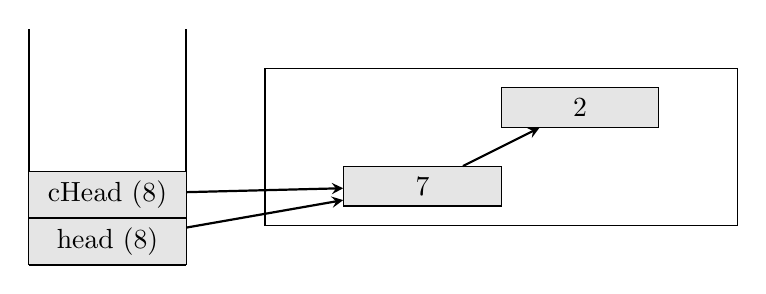
\begin{tikzpicture}
			\tikzstyle{Heap} = [rectangle, minimum width=6cm, minimum height=2cm, text centered, draw=black, fill=white]
			\tikzstyle{Stack} = [rectangle, minimum width=3cm, minimum height=1cm, text centered, draw=black, fill=white]
			\tikzstyle{ListNode} = [rectangle, minimum width=2cm, minimum height=5mm, text centered, draw=black, fill= gray!20]
			\tikzstyle{arrow} = [thick,->,>=stealth]
			
			%\foreach \x in {-2,-1,0,1,2,3,4}
			%	\draw (\x cm,1pt) -- (\x cm,-1pt) node[anchor=north] {$\x$};
			%\foreach \y in {-2,-1,0,1,2,3,4}
			%	\draw (1pt,\y cm) -- (-1pt,\y cm) node[anchor=east] {$\y$};
			%\draw[step=5mm,gray,very thin] (-2,-2) grid (6,6);
			
			\draw [thick, black] (-3, 0) -- (-1, 0);
			\draw [thick, black] (-3, 0) -- (-3, 3);
			\draw [thick, black] (-1, 0) -- (-1, 3);
			\node[Heap] at (3,1.5){};
			\node (7node) [ListNode] at (2,1) {7};
			\node (2node) [ListNode] at (4,2) {2};
			\node (cHeadNode) [ListNode] at (-2,0.9) {cHead (8)};
			\node (headNode) [ListNode] at (-2,0.3) {head (8)};
			\draw [arrow] (7node) -- (2node);
			\draw [arrow] (headNode) -- (7node);
			\draw [arrow] (cHeadNode) -- (7node);
		\end{tikzpicture}
	\end{center}
	%}
	
	Kerüljük ki a hibát, és írjunk saját copy konstruktort!
	
	
\begin{lstlisting}
struct List
{
	//...
	
	List(const List &other) : data(other.data), next(0)
	{
		if (other.next != 0)
		{
			next = new List(*other.next);
		}
	}
	
	//...
};

int main()
{
	List head(8);
	head.add(7);
	head.add(2);
	{
		List cHead = head;
	}
}
\end{lstlisting}
	Mint a korábbi függvényeink, ez is rekurzióval működik: a \texttt{new List(*other.next)} újra és újra meghívja a copy konstruktort, amíg az other.next nem lesz nullpointer.
	\begin{center}
		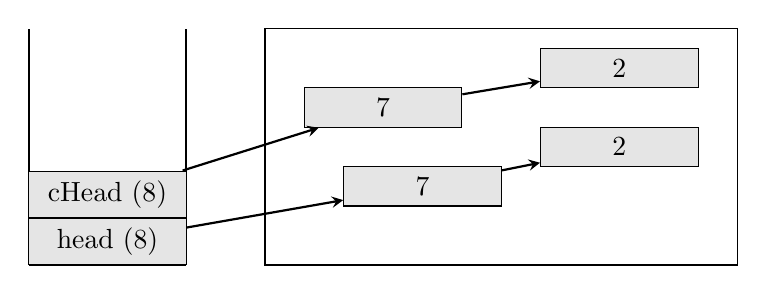
\begin{tikzpicture}
		\tikzstyle{Heap} = [rectangle, minimum width=6cm, minimum height=3cm, text centered, draw=black, fill=white]
		\tikzstyle{Stack} = [rectangle, minimum width=3cm, minimum height=1cm, text centered, draw=black, fill=white]
		\tikzstyle{ListNode} = [rectangle, minimum width=2cm, minimum height=5mm, text centered, draw=black, fill= gray!20]
		\tikzstyle{arrow} = [thick,->,>=stealth]
		
		%\foreach \x in {-2,-1,0,1,2,3,4}
		%	\draw (\x cm,1pt) -- (\x cm,-1pt) node[anchor=north] {$\x$};
		%\foreach \y in {-2,-1,0,1,2,3,4}
		%	\draw (1pt,\y cm) -- (-1pt,\y cm) node[anchor=east] {$\y$};
		%\draw[step=5mm,gray,very thin] (-2,-2) grid (6,6);
		
		\draw [thick, black] (-3, 0) -- (-1, 0);
		\draw [thick, black] (-3, 0) -- (-3, 3);
		\draw [thick, black] (-1, 0) -- (-1, 3);
		\node[Heap] at (3,1.5){};
		\node (7node) [ListNode] at (2,1) {7};
		\node (2node) [ListNode] at (4.5,1.5) {2};
		\node (7node2) [ListNode] at (1.5,2) {7};
		\node (2node2) [ListNode] at (4.5,2.5) {2};
		\node (cHeadNode) [ListNode] at (-2,0.9) {cHead (8)};
		\node (headNode) [ListNode] at (-2,0.3) {head (8)};
		\draw [arrow] (7node) -- (2node);
		\draw [arrow] (7node2) -- (2node2);
		\draw [arrow] (headNode) -- (7node);
		\draw [arrow] (cHeadNode) -- (7node2);
		\end{tikzpicture}
	\end{center}
	
	\medskip
	Ezzel meg is oldottuk a problémát. 
	
	Figyelem, ez egy \textbf{copy konstruktor, nem értékadás operátor!} Itt a \texttt{cHead} még nincs létrehozva, amikor head-el \textbf{inicializálni} próbáljuk. Ha az egyenlőségjel bal oldalán lévő objektum még nem jött létre, mint itt, akor a copy konstruktor hívódik meg. Ellenkező esetben értékadás operátor.
	\begin{lstlisting}
List cHead = head; //copy ctor

List cHead;
cHead = head; //ertekadas
	\end{lstlisting}
	
\end{document}
